% Dit werk is gelicenseerd onder de licentie Creative Commons Naamsvermelding-GelijkDelen 4.0 Internationaal. Ga naar http://creativecommons.org/licenses/by-sa/4.0/ om een kopie van de licentie te kunnen lezen.
\chapter{Leidingstelsels}
\label{sec:Leidingstelsels}

%%%%%%%%%%%%%%%%%%%%%%%%%%%%%%%%%%%%%%%%%%%%%%%%%%%%%%%%%%%%%%%%%%%%%%%%%%
	\section{Inleiding}
	\label{sec:Leidingstelsels Inleiding}
Ingenieurstoepassingen hebben vaak te maken met het transport van een fluïdum van één locatie naar een andere. Dit kan gebeuren in een leidingstelsel. In het voorgaande hoofdstuk hebben we reeds berekend welke drukverliezen veroorzaakt worden door de viskeuze spanningen in een horizontale leiding. Een praktisch leidingstelsel zal echter bestaan uit een aaneenschakeling van meerdere leidingen, bochten, veranderingen van diameter, kranen, aanzuigmonden, pompen,...

In dit hoofdstuk zullen we trachten enkele basis componenten van een leidingstelsel uit te lichten en te analyseren.

%%%%%%%%%%%%%%%%%%%%%%%%%%%%%%%%%%%%%%%%%%%%%%%%%%%%%%%%%%%%%%%%%%%%%%%%%%
	\section{Ladingsverliezen}
	\label{sec:Ladingsverliezen}
In het vorige hoofdstuk hebben we de drukverliezen van een viskeuze stroming in een leiding bepaald. Hierbij zijn we er telkens vanuit gegaan dat de viskeuze krachten in evenwicht waren met de drukkrachten. Het verschil in druk aan het begin en het einde van de leiding was met andere woorden de drijvende kracht van de stroming. Wanneer een leiding onder een helling staat zal de zwaartekracht echter ook een kracht uitoefenen op het fluïdum en dus een deel van de drijvende kracht vormen. We moeten het drukverlies uit het vorige hoofdstuk dus op een andere manier beschouwen. Dit kan door het te beschouwen als een energieverlies. Door de viscositeit zal een deel van de mechanische energie aanwezig in een stroming gedissipeerd worden. Het drukverlies uit het vorige hoofdstuk komt dus ook overeen met een energieverlies. Wanneer we de eenheden beschouwen zien we dat de eenheid [\unit{Pa}] inderdaad overeenkomt met een hoeveelheid energie per volume [\unit{J/m^3}].

In sectie \ref{sec:Mechanische arbeid van een deeltje} hebben we de vergelijking van Bernoulli beschouwd als behoud van mechanische energie van een niet-viskeuze, stationaire stroming langs een stroomlijn. In een leiding zullen er steeds stoomlijnen de leiding volgen. De precieze ligging van deze stroomlijnen in de leiding is niet belangrijk aangezien we in de gemiddelde grootheden overheen de leiding geïnteresseerd zijn. Bij viskeuze stromingen zal echter een deel van de mechanische energie verloren gaan. We kunnen (\ref{eqn:kinetische energie en arbeid}) dus herformuleren voor een viskeuze stroming:
\begin{equation}
	 \rho g z_2 + p_2 + \rho \frac{1}{2} v_2^2 =  \rho g z_1 + p_1 + \rho \frac{1}{2} v_1^2 - \Delta E
\end{equation}
Met $\Delta E$ het energieverlies ten gevolge van de viskeuze dissipatie zoals berekend in het vorige hoofdstuk. Een vaak gebruikte voorstelling van deze vergelijking is de weergave als energiehoogtes of ladingen. De lading (E: head) $H$ in een punt van een stroming is gedefinieerd als de totale mechanische energie in dat punt gedeeld door de valversnelling en de dichtheid in het punt:
\begin{equation}
	H = z + \frac{p}{\rho g} + \frac{v^2}{2 g}
\end{equation}
Als we de volledige mechanische energievergelijking delen door $\rho g$ kunnen we deze dus schrijven als:
\begin{equation}
	H_2 = H_1 - h_L
\end{equation}
Met $H_1$ de lading in punt $1$ en $H_2$ de lading in punt $2$.
De term $h_L$ wordt dan het \emph{ladingsverlies} (E: head loss) genoemd. In woorden stelt de vergelijking dat de lading in punt 2 gelijk is aan de lading in punt 1 min het ladingsverlies. De uitdrukking voor dit ladingsverlies in eenvoudig af te leiden uit (\ref{eqn:drukval bij turbulente stroming}) door te delen door $\rho g$:
\begin{equation}
	h_L = f \frac{v^2}{2 g} \frac{L}{D}
	\label{eqn:ladingsverlies door een leiding}
\end{equation}
In ingenieurstoepassingen zijn we vaak niet geïnteresseerd in de gemiddelde snelheid van de stroming in een leiding. We zijn geïnteresseerd in het debiet dat door deze leiding stroomt. Dit debiet kunnen we echter eenvoudig berekenen met behulp van de gemiddelde snelheid en de diameter als $\dot{V} = v \pi D^2/4$. We kunnen dus vergelijking (\ref{eqn:ladingsverlies door een leiding}) herschrijven als:
\begin{equation}
	h_L = 8 f \frac{\dot{V}^2}{g \pi^2} \frac{L}{D^5}
	\label{eqn:ladingsverlies door een leiding debiet}
\end{equation}

\begin{voorbeeld}
\label{ex:leiding tussen reservoirs}
Een leiding met cirkelvormige doorsnede en lengte 10 \unit{m}, diameter 0.10 \unit{m} en ruwheid 0.1 \unit{mm} verbind twee waterreservoirs. De niveau's van deze reservoirs worden op constante hoogte gehouden en het hoogteverschil tussen de twee reservoirs is 1 \unit{m}. 

Bepaal het debiet door de leiding.

We kunnen de mechanische energie vergelijking opschrijven tussen twee punten met punt $1$ aan het oppervlak van het hoger gelegen reservoir en punt $2$ aan het oppervlak van het lager gelegen reservoir. 
\begin{equation}
	H_2 = H_1 - h_\mathrm{L} \nonumber
\end{equation}

In beide punten is de snelheid bij benadering gelijk aan nul, en de druk atmosfeerdruk. De lading in punt 1 en 2 is dus gelijk aan het niveau van de waterreservoirs. Bovenstaande vergelijking vereenvoudigt zich dus tot:
\begin{equation}
	z_1 - z_2 = h_\mathrm{L}
	\label{eqn:voorbeeld leiding tussen reservoirs energie}
\end{equation}

De ladingsverliezen kunnen verder uitgeschreven worden als:
\begin{equation}
	h_\mathrm{L} = 8 f \frac{\dot{V}^2}{\pi^2 g}\frac{L}{D^5}
\end{equation}

Op de wrijvingsfactor te bepalen uit figuur \ref{fig:Moody diagram} hebben we het Reynoldsgetal nodig. Dit kunnen we bepalen uit het debiet als:
\begin{equation}
	\mathrm{Re} = \frac{v D}{\nu} = \frac{4 \dot{V}}{\pi D \nu}
\end{equation}

De wrijvingsfactor kan niet rechtstreeks bepaald worden aangezien deze afhankelijk is van het Reynoldsgetal en dus ook van het nog onbekende debiet. Om een oplossing te bekomen gebruiken we dus een iteratieve oplossingsprocedure:
\begin{enumerate}
	\item schat $f$
	\item los (\ref{eqn:voorbeeld leiding tussen reservoirs energie}) op naar $\dot{V}$
	\item bepaal $\mathrm{Re}$ met het gevonden debiet
	\item bepaal $f$ met behulp van het Moody diagram
	\item ga naar stap 2
\end{enumerate}

Indien we beginnen van een veronderstelling $f=0.030$ bekomen we de volgende oplossingstabel:
\begin{center}
	\begin{tabular}{llll}
		\hline
		iteratie & $\mathrm{Re}$   & $f$   & $\dot{V}$ (\unit{m^3/s}) \\
		\hline
		0        &       /         & 0.030 &  $0.0201$ \\
		1        & $256\times10^3$ & 0.021 &  $0.0242$ \\
		2        & $308\times10^3$ & 0.021 &  $0.0243$ \\
		\hline
	\end{tabular}
\end{center}

Het debiet door de leiding is dus 0.024 \unit{m^3/s}

\end{voorbeeld}


%%%%%%%%%%%%%%%%%%%%%%%%%%%%%%%%%%%%%%%%%%%%%%%%%%%%%%%%%%%%%%%%%%%%%%%%%%
	\section{Lokale ladingsverliezen}
	\label{sec:Lokale ladingsverliezen}
Wanneer een fluïdum door een kraan stroomt zal er een bepaald ladingsverlies optreden ten gevolge van de stand van de kraan. Aangezien dit ladingsverlies, in tegenstelling tot het ladingsverlies in een leiding, aan één specifieke locatie kan toegewezen worden wordt er gesproken over lokale ladingsverliezen. Voor de meeste componenten is het moeilijk de lokale ladingsverliezen analytisch te bepalen. Voor de bepaling ervan wordt vaak gebruik gemaakt van een empirisch bepaalde verliescoëfficiënt gedefinieerd zodat:
\begin{equation}
	h_{L, lokaal} = K \frac{v^2}{2 g} = K \frac{\dot{V}^2}{2 g A^2}
	\label{eqn:lokale ladingsverliezen}
\end{equation}
Uit dimensie analyse blijkt dat de verliescoëfficiënt een functie moet zijn van de geometrie en het Reynoldsgetal.
\begin{equation}
	K = K(geometrie, Re)
\end{equation}
In vele gevallen zal de invloed van het Reynoldsgetal echter verwaarloosd kunnen worden. Dit komt omdat in kranen, bochten,... de energieverliezen voornamelijk veroorzaakt worden door richtingsveranderingen (traagheidskrachten) in in mindere mate door viskeuze krachten. Bij een bocht kunnen we bijvoorbeeld het ladingsverlies opsplitsen in een ladingsverlies ten gevolge van de richtingsverandering (Reynolds onafhankelijk) en een ladingsverlies ten gevolge van de lengte van de bocht (Reynolds afhankelijk). Het ladingsverlies ten gevolge van de lengte van de bocht kan berekend worden met behulp van de formules voor een rechte leiding en wordt dan ook meestal bij de gewone ladingsverliezen gerekend.

De waarden van de verliescoëfficiënt voor enkele veel voorkomende leidingsonderdelen zijn gegeven in Appendix \ref{sec:Tabellen en grafieken}.

De lokale ladingsverliezen worden ook soms uitgedrukt als een equivalente leiding lengte. De component wordt dan beschouwd als een extra deel leiding met dezelfde diameter als de leiding waarin het is ingebouwd dat hetzelfde ladingsverlies zou veroorzaken als de werkelijke component. De equivalente lengte wordt dan:
\begin{equation}
	L_{equivalent} = \frac{K D}{f}
\end{equation}

Uit (\ref{eqn:lokale ladingsverliezen}) blijkt dat we de verliescoëfficiënt beschouwen als de fractie van de kinetische energie van de stroming die in de beschouwde component verloren gaat. Om dit te illustreren zullen we de verliescoëfficiënt bij een plotse verwijding bepalen. Dit is één van de weinige leidingsonderdelen waarvoor het ladingsverlies analytisch kan uitgerekend worden.

	\subsection{Ladingsverlies bij een plotse verwijding}
Beschouw een plotse verwijding in een leiding als in Figuur \ref{fig:Plotse verwijding}. Ter hoogte van de verwijding zal er een jet-achtige stroming ontstaan. Voldoende verderop zal de stroming opnieuw volledig ontwikkeld zijn. Beschouwen we nu een impulsbalans voor het aangeduide controlevolume.
\begin{figure}
	\centering
	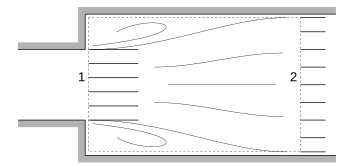
\includegraphics{fig/leidingstelsels/Plotse_verwijding}
	\caption{Plotse verwijding in een leiding}
	\label{fig:Plotse verwijding}
\end{figure}
Ter hoogte van de ingang lopen alle stroomlijnen parallel. Er kan dus geen drukverandering zijn loodrecht op de stroomlijnen. De druk op de linkerzijde van het controlevolume is met andere woorden constant en gelijk aan de druk vlak voor de verwijding. Indien we een uniforme snelheid veronderstellen (Geldig bij zeer hoge Reynoldsgetallen) aan de instroming en uitstroming bekomen we:
\begin{equation}
	p_1 A_2 - p_2 A_2 = \rho A_2 v_2 (v_2-v_1)
\end{equation}
De energie vergelijking wordt hier:
\begin{equation}
	\frac{p_2}{\rho g} + \frac{v_2^2}{2 g} = \frac{p_1}{\rho g} + \frac{v_1^2}{2 g} - h_L
\end{equation}
Wanneer we deze twee vergelijkingen combineren bekomen we:
\begin{equation}
	h_L = \frac{v_1^2}{2 g} \left(1 - 2\frac{v_2}{v_1} + \frac{v_2^2}{v_1^2} \right)
\end{equation}
Indien we hierin de verhouding van snelheden vervangen door de verhouding van oppervlaktes (behoud van massa) verkrijgen we:
\begin{equation}
	h_L = \frac{v_1^2}{2 g} \left(1 - \frac{A_1}{A_2} \right)^2
\end{equation}
De verliescoëfficiënt wordt dus:
\begin{equation}
	K = \left(1 - \frac{A_1}{A_2} \right)^2
\end{equation}
De verliescoëfficiënt is hier dus enkel een functie van de geometrie. Dit resultaat is in goede overeenstemming met experimenteel bepaalde waarden. Wanneer we de oppervlakte $A_2$ naar oneindig laten gaan bekomen we de verliescoëfficiënt voor een uitstroming in een zeer groot reservoir. De verliescoëfficiënt is dan 1. Met andere woorden de volledige kinetische energie wordt gedissipeerd tijdens de uitstroming in een reservoir.

\begin{voorbeeld}
\label{ex:voorbeeld leiding tussen reservoirs lokale verliezen}
Bepaal voor het systeem uit  voorbeeld \ref{ex:leiding tussen reservoirs} het debiet door de leiding rekeninghoudend met de ladingsverliezen aan in- en uitstroom als de in- en uitstroom van de leiding in de reservoirs zonder afrondingen is uitgevoerd.

We kunnen de mechanische energie vergelijking (\ref{eqn:voorbeeld leiding tussen reservoirs energie}) uit voorbeeld \ref{ex:leiding tussen reservoirs} uitbreiden door de lokale verliezen toe te voegen:
\begin{equation}
	z_1 -z_2 = h_\mathrm{L} + h_\mathrm{L,instroom} + h_\mathrm{L,uitstroom}
	\label{eqn:voorbeeld leiding tussen reservoirs lokale verliezen energie}
\end{equation}

De lokale ladingsverliezen kunnen verder uitgeschrenen worden als:
\begin{align}
	h_\mathrm{L,instroom} &= 8 K_\mathrm{instroom} \frac{\dot{V}^2}{\pi^2 g D^4} \nonumber \\
	h_\mathrm{L,uitstroom} &= 8 K_\mathrm{uitstroom} \frac{\dot{V}^2}{\pi^2 g D^4} \nonumber
\end{align}

De verliescoëfficiënten $K_\mathrm{instroom}$ en $K_\mathrm{uitstroom}$ kunnen we bekomen uit Appendix \ref{sec:Tabellen en grafieken}. Voor de niet afgeronde in- en uitstroom wordt dit:
\begin{align}
	K_\mathrm{instroom} = 0.5 \nonumber \\
	K_\mathrm{uitstroom} = 1.0 \nonumber
\end{align}

Om een oplossing te bekomen kan dezelfde iteratieve oplossingsprocedure als in voorbeeld \ref{ex:leiding tussen reservoirs} gebruikt worden. Indien we opnieuw beginnen van een veronderstelling $f=0.030$ bekomen we de volgende oplossingstabel:
\begin{center}
	\begin{tabular}{llll}
		\hline
		iteratie & $\mathrm{Re}$   & $f$   & $\dot{V}$ (\unit{m^3/s}) \\
		\hline
		0        &       /         & 0.030 &  $0.0164$ \\
		1        & $209\times10^3$ & 0.021 &  $0.0183$ \\
		2        & $234\times10^3$ & 0.021 &  $0.0184$ \\
		\hline
	\end{tabular}
\end{center}

Het debiet door de leiding is dus 0.018 \unit{m^3/s}

\end{voorbeeld}

%%%%%%%%%%%%%%%%%%%%%%%%%%%%%%%%%%%%%%%%%%%%%%%%%%%%%%%%%%%%%%%%%%%%%%%%%%
	\section{Serie en parallelschakeling van leidingen}
	\label{sec:Serie en parallelschakeling van leidingen}
Aangezien leidingstelsels niet uit enkelvoudige rechte leidingen bestaan maar een vaak veel complexere structuur hebben (zie Figuur \ref{fig:leiding_structuur}), is het aangewezen deze structuur op te delen in enkele basis bouwstenen. De eenvoudigste van deze bouwstenen is de serie schakeling van elementen.
\begin{figure}
	\centering
	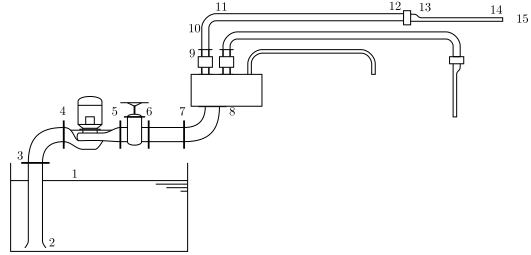
\includegraphics{fig/leidingstelsels/leiding_structuur}
	\caption{Voorbeeld van een leidingstructuur}
	\label{fig:leiding_structuur}
\end{figure}
Bij een serie schakeling (Figuur \ref{fig:serieschakeling}) zal logischerwijze het totale ladingsverlies gelijk zijn aan de som der ladingsverliezen. Voor een serieschakeling van $n$ componenten kunnen we dus schrijven:
\begin{equation}
h_{L,serie} = \sum_i^n h_{L,i}
\end{equation}
Aangezien het debiet in alle componenten gelijk is wordt dit voor een serieschakeling van leidingen:
\begin{equation}
	h_{L,serie} = \sum_i^n 8 f_i \frac{\dot{V}^2}{g \pi^2} \frac{L_i}{D^5_i}
	\label{eqn:ladingsverlies door leidingen in serie}
\end{equation}
\begin{figure}
	\centering
	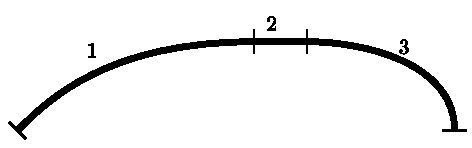
\includegraphics{fig/leidingstelsels/serieschakeling}
	\caption{Serieschakeling van componenten}
	\label{fig:serieschakeling}
\end{figure}

Een iets complexere structuur is de parallelschakeling (\ref{fig:parallelschakeling}). Bij een parallelschakeling van leidingen zal de stroming zich opsplitsen tussen de verschillende elementen. Het totale ladingsverlies tussen het begin en het einde van de parallelschakeling kunnen we bekomen door op te merken dat het ladingsverlies door elk van de elementen die deel uitmaken van de schakeling hetzelfde ladingsverlies moeten veroorzaken. Het totaal debiet zal dus zodanig opgesplitst worden dat het ladingsverlies in alle componenten gelijk is:
\begin{figure}
	\centering
	\includegraphics{fig/leidingstelsels/parallelschakeling}
	\caption{Parallelschakeling van componenten}
	\label{fig:parallelschakeling}
\end{figure}
\begin{equation}
	h_{L,parallel} = h_{L,i} \quad i=1..n
\end{equation}
Voor een parallelschakeling van leidingen wordt dit:
\begin{equation}
	h_{L,parallel} = 8 f_i \frac{\dot{V_i}^2}{g \pi^2} \frac{L_i}{D^5_i} \quad i=1..n
\end{equation}
Samen met de continuïteitsvergelijking levert dit een stelsel van $n+1$ vergelijkingen en $n+1$ onbekenden ($h_{L,parallel}$ en $\dot{V}_i, i=1..n$):
\begin{equation}
	\left\{
	\begin{array}{lcl}
		h_{L,parallel} &=& 8 f_i \frac{\dot{V_i}^2}{g \pi^2} \frac{L_i}{D^5_i} \quad i=1..n \\
		\dot{V} &=& \sum_i^n \dot{V}_i
	\end{array}
	\right.
	\label{eqn:parallelschakeling}
\end{equation}

%%%%%%%%%%%%%%%%%%%%%%%%%%%%%%%%%%%%%%%%%%%%%%%%%%%%%%%%%%%%%%%%%%%%%%%%%%
	\section{Leiding netwerken}
	\label{sec:Leiding netwerken}	
Niet alle structuren van leidingen kunnen opgesplitst worden in eenvoudige serie- en parallelschakelingen zoals hierboven beschreven. In Figuur \ref{fig:leidingnetwerk} is een leiding structuur gegeven met slechts drie leidingen die niet als een serie- of parallelschakeling kan beschouwd worden. Zo'n structuur noemen we een leidingnetwerk.
\begin{figure}
	\centering
	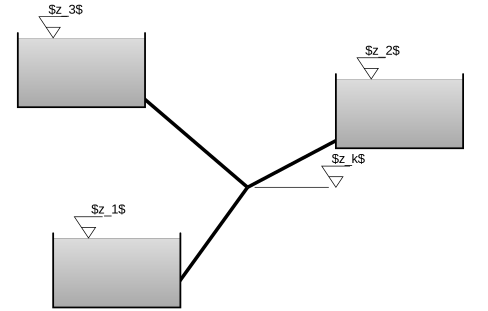
\includegraphics{fig/leidingstelsels/Leidingnetwerk}
	\caption{Leiding netwerk}
	\label{fig:leidingnetwerk}
\end{figure}
Indien we de leidingen vertrekkende uit reservoir $i$ aanduiden met de index $i$ kunnen we voor dit systeem met zekerheid 3 stroomlijnen tekenen. Namelijk de stroomlijnen vertrekkende van het oppervlak van reservoir $i$ en aankomend in het knooppunt. Voor elk van deze stroomlijnen kunnen we de energievergelijking uitschrijven:
\begin{equation}
	\left\{
	\begin{array}{lcl}
		H_k &=& H_1 - h_{L,1} \nonumber \\
		H_k &=& H_2 - h_{L,2} \\
		H_3 &=& H_k - h_{L,3} \nonumber
	\end{array}
	\right.
\end{equation} 
Bij het opschrijven van deze vergelijkingen hebben we impliciet stroomrichtingen verondersteld. In leiding 1 en 2 hebben de stroming naar het knooppunt toe verondersteld, terwijl in leiding 3 de stroming van het knooppunt weg verondersteld is. De ladingsverliezen kunnen we ook schrijven in functie van de debieten in de 3 leidingen. Indien we de wrijvingsfactoren gekend veronderstellen (wat mogelijk is door het gebruik van een iteratieve techniek) hebben we dus een stelsel van 3 vergelijkingen en 4 onbekenden ($\dot{V}_1,\dot{V}_2,\dot{V}_3$ en $H_k$). Er is dus nog één vergelijking nodig om dit stelsel te kunnen oplossen. Deze vinden we in de vorm van de continuïteitsvergelijking. In het knooppunt moet namelijk evenveel massa toekomen als vertrekken. Het volledige stelsel wordt dus:
\begin{equation}
	\left\{
	\begin{array}{lcl}
		H_k &=& H_1 - 8 f_1 \dfrac{\dot{V}_1^2}{g \pi^2} \dfrac{L_1}{D_1^5} \\
		H_k &=& H_2 - 8 f_2 \dfrac{\dot{V}_2^2}{g \pi^2} \dfrac{L_2}{D_2^5} \\
		H_3 &=& H_k - 8 f_3 \dfrac{\dot{V}_3^2}{g \pi^2} \dfrac{L_3}{D_3^5} \\
		\dot{V}_3 &=& \dot{V}_1 + \dot{V}_2
	\end{array}
	\right.
	\label{eqn:3reservoirs stelsel}
\end{equation}
Bij het opstellen van deze vergelijkingen is voor de 3 leidingen reeds een stroomrichting verondersteld. Er wordt namelijk verondersteld dat de stroming van 1 en 2 naar het knooppunt gaat en van het knooppunt naar 3. Dit stelsel van vergelijkingen is dus enkel geldig indien achteraf ook blijkt dat de stromingen in deze richting lopen. Dit komt erop neer dat de gebruikte debieten $V_1$,$V_2$ en $V_3$ allen groter dan nul moeten zijn.

Aangezien 3 van de 4 vergelijkingen in het stelsel (\ref{eqn:3reservoirs stelsel}) kwadratisch zijn in het onbekende debiet, zal het stelsel meer dan één oplossing hebben. Indien het stelsel met behulp van analytische rekensoftware wordt opgelost zullen al deze oplossingen weergegeven worden. Het is dan aan de probleemoplosser op de juiste oplossing te selecteren. De juiste oplossing moet namelijk voldoen aan de hierboven genoemde voorwaarde, alle debieten moeten groter dan nul zijn.

Het is echter ook mogelijk dat de oplossing van het bovenstaande stelsel geen enkele oplossing geeft waarvoor alle debieten groter zijn dan nul. Geen enkel van de oplossingen van het stelsel geeft dan de gezochte debieten aangezien het stelsel niet meer geldig is.

Wanneer dit voorvalt wil het zeggen dat één of meerdere stromingsrichtingen verkeerd gekozen zijn. We moeten dus het stelsel aanpassen zodat het overeenkomt met een nieuwe veronderstelling voor de stroomrichtingen.

In het geval van Figuur \ref{fig:leidingnetwerk} is het, afhankelijk van de getalwaarden voor de hoogtes, leiding lengtes en diameters, best mogelijk dat de stroming niet van punt 2 naar het knooppunt gaat, maar van het knooppunt naar punt 2. We moeten dan de energievergelijking tussen punt 2 en het knooppunt en de continuïteitsvergelijking aanpassen:
\begin{equation}
	\left\{
	\begin{array}{lcl}
		H_k &=& H_1 - 8 f_1 \dfrac{\dot{V}_1^2}{g \pi^2} \dfrac{L_1}{D_1^5} \\
		H_2 &=& H_k - 8 f_2 \dfrac{\dot{V}_2^2}{g \pi^2} \dfrac{L_2}{D_2^5} \\
		H_3 &=& H_k - 8 f_3 \dfrac{\dot{V}_3^2}{g \pi^2} \dfrac{L_3}{D_3^5} \\
		\dot{V}_3 + \dot{V}_2 &=& \dot{V}_1 
	\end{array}
	\right.
	\label{eqn:3reservoirs stelsel2}
\end{equation}

Met dit nieuwe stelsel van vergelijkingen kan nu wel een correcte oplossing, waarvoor alle 3 de debieten groter zijn dan nul bekomen worden.

%%%%%%%%%%%%%%%%%%%%%%%%%%%%%%%%%%%%%%%%%%%%%%%%%%%%%%%%%%%%%%%%%%%%%%%%%%
	\section{Stromingsweerstand oplossingsmethode}
	\label{sec:stromingsweerstand oplossingsmethode}
voor het bepalen van de debieten in zelfs eenvoudige leidingstelsels ontstaan stelsels waarin lineaire vergelijkingen en kwadratische vergelijkingen door elkaar staan. De uitdrukking van de mechanische energievergelijking tussen twee punten in een leiding geeft namelijk een vergelijking die kwadratisch is in het debiet door de leiding. De continuïteitsvergelijking in een knooppunt geeft dan weer een vergelijking die lineair is in de debieten. Bovendien is de wrijvingsfactor ook zee niet lineair afhankelijk van het debiet. Het oplossen van zo'n stelsel is niet voor de hand liggend en vaak zijn numerieke oplossingstechnieken de enige uitweg.

We kunnen de oplossing echter een stukje vereenvoudigen indien we het begrip stromingsweerstand invoeren naar analogie met een elektrische weerstand. We zouden namelijk de mechanische energievergelijking kunnen schrijven als:
\begin{equation}
	H_2 = H_1 - R \dot{V}			
\end{equation}
Hierin kunnen we $R$ de stromingsweerstand van een leiding uitschrijven als:
\begin{equation}
	R = 8 f \dfrac{|\dot{V}|}{g \pi^2} \dfrac{L}{D^5}	
\end{equation}
Voor een lokaal verlies wordt dit:
\begin{equation}
	R_\mathrm{lokaal} = K \frac{|\dot{V}|}{2 g A^2}
\end{equation}

Indien we de waarden van de stromingsweerstanden kennen bekomen we dan een stelsel met enkel nog lineaire vergelijkingen waarin de debieten en ladingen in interne knooppunten onbekend zijn. Dit stelsel kan dus eenvoudig opgelost worden.
De stromingsweerstanden zijn echter ook functies van het debiet. We kunnen ze dus niet a priori bepalen. Er moet dus eerst een veronderstelling gemaakt worden omtrent de debieten. Met deze veronderstelling kunnen wrijvingsfactoren en de waarden van de stromingsweerstanden bepaald worden. Eens deze vast liggen kan het stelsel dat volgt uit de mechanische energievergelijkingen en de continuïteitsvergelijkingen opgelost worden naar de onbekende debieten. Deze debieten kunnen dan gebruikt worden om nieuwe, betere waarden voor de stromingsweerstanden te bepalen en de procedure kan herhaald worden tot de bekomen oplossing convergeert.

Voor serie en parallelschakelingen van leidingen heeft het werken met stromingsweerstanden nog een bijkomend voordeel. Aangezien de mechanische energievergelijking analoog is aan de wet van Ohm, kunnen de vergelijkingen voor de totale weerstand van een serie of parallelschakeling ook gebruikt worden in een stromingsprobleem.

Voor een serieschakeling van leidingen zal de totale weerstand dus de som van de weerstanden van de onderdelen zijn:
\begin{equation}
	R_\mathrm{serie} = \sum_i R_i
\end{equation}
Voor een parallelschakeling van leidingen is de inverse van de totale weerstand gelijk aan de som van de inversen van de weerstanden van onderdelen:
\begin{equation}
	R_\mathrm{parallel} = \left( \sum_i \frac{1}{R_i} \right)^{-1}
\end{equation}

Met deze uitdrukkingen kan dus voor een systeem dat bestaat uit serie en parallelschakelingen van verschillende componenten, de totale stromingsweerstand van het systeem bepaald worden. Het oplossen van een stelsel is dan zelfs niet meer nodig aangezien er slechts één vergelijking overblijft.


%%%%%%%%%%%%%%%%%%%%%%%%%%%%%%%%%%%%%%%%%%%%%%%%%%%%%%%%%%%%%%%%%%%%%%%%%%
	\section{Types stromingsproblemen}
	\label{sec:types stromingsproblemen}
Bij het toepassen van bovenstaande uitdrukkingen op ingenieurstoepassingen ontstaan er meteen enkele verscillende types toepassingen. Wanneer de debieten in de leidingen gekend zijn kunnen we met behulp van het Moody diagram de ladingsverliezen (en dus de drukken in elk punt van de leidingen) berekenen. Dit is echter niet het enige type probleem dat we kunnen tegenkomen. Algemeen zijn er drie types problemen te onderscheiden:
\begin{itemize}
	\item Het berekenen van ladingsverliezen uit het debiet en de geometrie
	\item Het berekenen van het debiet uit gekende ladingsverliezen en geometrie
	\item Het berekenen van de geometrie met gekende ladingsverliezen bij een bepaald debiet
\end{itemize}
Het eerste type toepassingen is zeer eenvoudig en kan bij een serieschakeling van elementen zonder problemen gedaan worden. Wanneer er echter een parallelschakeling in het leidingstelsel voorkomt wordt ook dit probleem iets ingewikkelder. Naar alle waarschijnlijkheid zal de debietverdeling in de verschillende componenten van de parallelschakeling niet gekend zijn. We dienen dus het stelsel (\ref{eqn:parallelschakeling}) op te lossen. Hierin zijn de wrijvingsfactoren $f_i$ echter afhankelijk van het Reynoldsgetal en dus het debiet (dat niet gekend is). Bij turbulente stroming is deze relatie zelfs sterk niet lineair en moeilijk in gesloten vorm weer te geven. Daarbovenop is het stelsel (\ref{eqn:parallelschakeling}) zelf ook niet lineair. Er is dus geen garantie dat er een oplossing bestaat.
Indien de oplossing echter wel bestaat kunnen we met behulp van iteratieve technieken wel tot deze oplossing komen. Een stappenplan om tot een oplossing te komen gaat als volgt:
\begin{enumerate}
	\item Maak een veronderstelling voor het debiet in de verschillende leidingen
	\item Bereken de Reynoldsgetallen en de wrijvingsfactoren voor elke leiding met behulp van het Moody diagram
	\item Los het stelsel (\ref{eqn:parallelschakeling}) op naar de debieten met de veronderstelde wrijvingsfactoren
	\item Indien de debieten sterk afwijken van de voorgaande debieten ga naar stap 2, indien niet is de oplossing gevonden.
\end{enumerate}

Voor het tweede type toepassingen (Bepaling van het debiet bij een gekend ladingsverlies) kan bovenstaande oplossingsmethode ook gebruikt worden. Dit type problemen komt voor bij stroming die wordt veroorzaakt door hoogteverschillen tussen 2 reservoirs of bij stroming tussen een leiding op gekende druk en een reservoir. 

Het derde type toepassing is een typische ingenieursprobleem waarbij een bepaald debiet fluïdum van een locatie naar een andere getransporteerd dient te worden. De diameter van de leidingen moet zo gekozen worden dat het ladingsverlies over elk onderdeel beperkt blijft. Het toegelaten ladingsverlies bepaalt hoeveel vermogen er nodig is voor het transport en dus de grootte van pompen of ventilatoren en de energie nodig voor het transport. Aangezien het Reynoldsgetal (en dus ook de wrijvingsfactor) ook afhankelijk is van de diameter van de leiding, hebben we opnieuw een iteratieve techniek nodig om dit probleem op te lossen. Indien we het bovenstaande stappenplan licht aanpassen bekomen we:
\begin{enumerate}
	\item Maak een veronderstelling voor de diameter van de leiding
	\item Bereken de Reynoldsgetallen en de wrijvingsfactoren voor elke leiding met behulp van het Moody diagram
	\item Bepaal met behulp van (\ref{eqn:ladingsverlies door een leiding debiet}) de diameter
	\item Indien de diameters sterk afwijken van de voorgaande waarden ga naar stap 2, indien niet is de oplossing gevonden.
\end{enumerate}
Aangezien de diameters van leidingen sterk genormeerd zijn kan de eerstvolgende grotere leiding gekozen worden en dienen er nooit veel iteraties uitgevoerd te worden.


%%%%%%%%%%%%%%%%%%%%%%%%%%%%%%%%%%%%%%%%%%%%%%%%%%%%%%%%%%%%%%%%%%%%%%%%%%
	\section{Pomp - ventilator - leiding karakteristiek}
	\label{sec:Pomp - ventilator - leiding karakteristiek}
In de voorgaande secties werd het debiet in een leiding of leidingstelsel veroorzaakt door een hoogteverschil of het debiet werd verondersteld gekend te zijn. Het is echter ook mogelijk dat het de stroming wordt veroorzaakt door een pomp of ventilator. Dit zijn toestellen met als doel een bepaald debiet te genereren. Een pomp of ventilator zal dus net zoveel energie aan de stroming toevoegen totdat de toegevoegde energie gelijk is aan de energie die nodig is om hoogte of drukverschillen te overwinnen en de gedisipeerde energie. We kunnen de vergelijking van Bernoulli dus nogmaals uitbreiden naar situatie waar er energie aan de stroming toegevoegd wordt. Dit geeft: 
\begin{equation}
	H_2 = H_1 - h_L + h_P
	\label{eqn:mechanische energievergelijking}
\end{equation}
Hierin stelt $h_P$ de opvoerhoogte van de aanwezige pompen voor. De opvoerhoogte van een pomp is een maat voor de energie die de pomp aan de stroming toegevoegd. Vaak komt deze tot uiting als een drukverhoging van de inlaat tot de uitlaat van de pomp. Indien de we de hoogteverschillen en verschillen in kinetische energie tussen inlaat en uitlaat verwaarlozen vinden we het drukverschil tussen in en uitlaat als:
\begin{equation}
	\Delta p = \rho g h_P
\end{equation}
Vergelijking (\ref{eqn:mechanische energievergelijking}) wordt ook wel de mechanische energievergelijking genoemd.

Pompen kunnen we praktisch onderverdelen in twee types: \emph{Volumetrische pompen} en \emph{Turbopompen}. Bij volumetrische pompen (E: Positive displacement pump) zal er steeds een vast volume vloeistof verplaatst worden onafhankelijk van het drukverschil tussen in en uitlaat. Het meest voor de hand liggende voorbeeld is de zuigerpomp waar een zuiger of plunjer in samen werking met enkele kleppen voor de verplaatsing van de vloeistof zorgt. Een schets van het werkingsprincipe van een zuigerpomp is gegeven in Figuur \ref{fig:zuigerpomp} 
\begin{figure}
	\centering
	\subfigure[Zuigerpomp]{
		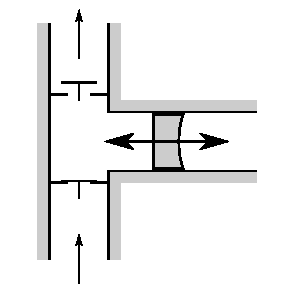
\includegraphics{fig/leidingstelsels/Zuigerpomp}
		\label{fig:zuigerpomp}
	} \quad
	\subfigure[Centrifugaalpomp]{
		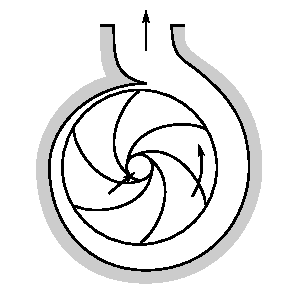
\includegraphics{fig/leidingstelsels/Centrifugaalpomp}
		\label{fig:centrifugaalpomp}
	}	
	\caption{Schematische voorstelling van een zuiger- en centrifugaalpomp}
	\label{fig:pompen}
\end{figure}

Bij een turbopomp zal er door middel van een rotor eerst kinetische energie aan de stroming toegevoegd worden. Nadien wordt deze kinetische energie in een diffusor omgezet naar druk energie. Een typische voorbeeld is de centrifugaal pomp (Figuur \ref{fig:centrifugaalpomp}). Vloeistof treedt binnen door een centrale opening. De stroming wordt door een rotor met schoepen radiaal naar buiten versneld waarna de bekomen kinetische energie in de diffusor in de vorm van een slakkenhuis wordt omgezet in druk.

Bij een turbopomp zal de geleverde opvoerhoogte wel afhankelijk zijn van het debiet. De relatie tussen de twee wordt vaak weergegeven in een pompkarakteristiek. Dit is een grafiek met op de $x$-as het debiet en op de $y$-as de opvoerhoogte. Vaak worden er verschillende krommen gegeven voor de werking bij verschillende toerentallen. Een voorbeeld van een pompkarakteristiek voor een centrifugaal pomp is gegeven in Figuur \ref{fig:Pompkarakteristiek}. De algemene trend is dat bij turbopompen de opvoerhoogte daalt bij stijgend debiet. Het is ook mogelijk een pompkarakteristiek te tekenen voor een volumetrische pomp. Dit is een verticale lijn bij het debiet dat de pomp levert. De opvoerhoogte is namelijk onafhankelijk van het debiet.
\begin{figure}
	\centering
	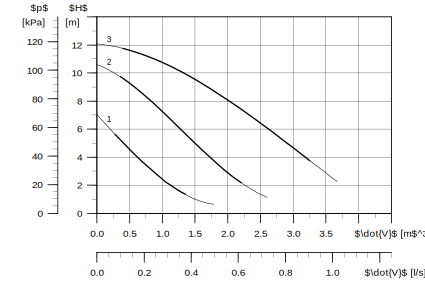
\includegraphics{fig/leidingstelsels/Pompkarakteristiek_UPS_25_120}
	\caption{Voorbeeld van een pompkarakteristiek van een centrifugaalpomp}
	\label{fig:Pompkarakteristiek}
\end{figure}

Ook voor het leidingstelsel kunnen we de nodige opvoerhoogte uitzetten in functie van het debiet. Deze kromme noemen we de leidingskarakteristiek. Indien we veronderstellen dat de wrijvingsfactor niet sterk verandert zien we uit vergelijking (\ref{eqn:ladingsverlies door een leiding debiet}) dat het ladingsverlies evenredig is met het kwadraat van het debiet. Een leidingskarakteristiek zal er dus kwalitatief uitzien als in Figuur \ref{fig:Leidingskarakteristiek}.
\begin{figure}
	\centering
	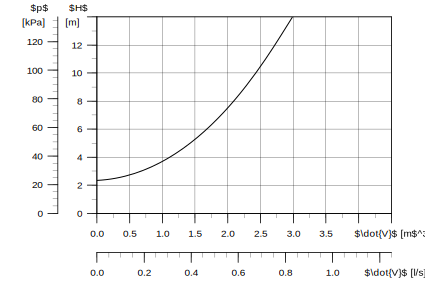
\includegraphics{fig/leidingstelsels/Leidingskarakteristiek}
	\caption{Voorbeeld van een leidingskarakteristiek}
	\label{fig:Leidingskarakteristiek}
\end{figure}
Wanneer we de pompkarakteristiek (Figuur \ref{fig:Pompkarakteristiek}) en leidingskarakteristiek (\ref{fig:Leidingskarakteristiek}) combineren kunnen we het werkingspunt van het systeem aflezen als het snijpunt van de twee krommen (Figuur \ref{fig:Pompleidingkarakteristiek}). In dit punt zal de opvoerhoogte geleverd door de pomp net gelijk zijn aan de energie nodig om her fluïdum door de leiding te verplaatsen.
\begin{figure}
	\centering
	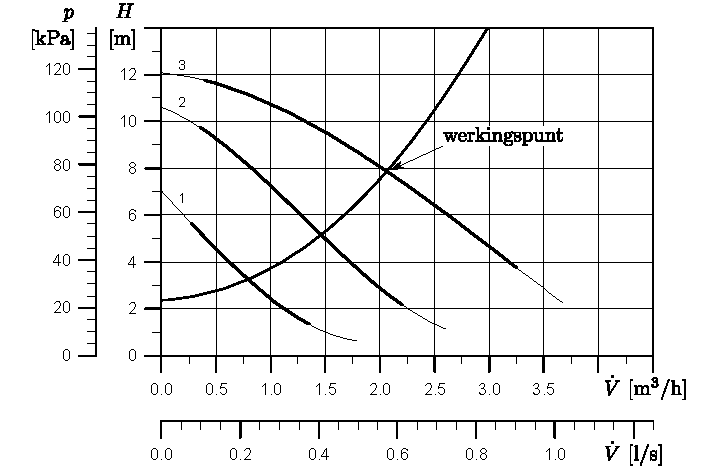
\includegraphics{fig/leidingstelsels/Pompleidingkarakteristiek}
	\caption{De combinatie van pomp en leidingskarakteristiek leidt tot het werkingspunt}
	\label{fig:Pompleidingkarakteristiek}
\end{figure}
Het zoeken van het werkingspunt op deze manier komt neer op het grafisch oplossen van de mechanische energievergelijking. De pompkarakteristiek en leidingskarakteristiek kunnen we namelijk schrijven als:
\begin{align}
	h_P(\dot{V}) \\
	H_2-H_1 + h_L(\dot{V})
\end{align}
Indien we deze twee aan elkaar gelijkstellen bekomen we de mechanische energievergelijking die we kunnen oplossen naar $\dot{V}$ om het werkingspunt te vinden.

%%%%%%%%%%%%%%%%%%%%%%%%%%%%%%%%%%%%%%%%%%%%%%%%%%%%%%%%%%%%%%%%%%%%%%%%%%
		\section{Grafische voorstelling}
In sectie \ref{sec:Mechanische arbeid van een deeltje} zijn we reeds een grafische voorstelling van de vergelijking van Bernoulli tegengekomen. We kunnen dezelfde grafische voorstelling ook maken voor de mechanische energievergelijking toegepast op een enkelvoudig leidingstelsel (langs één stoomlijn). De totale energiehoogte of ladingslijn zal nu echter niet meer horizontaal lopen. Ten gevolge van ladingsverliezen in leidingen of lokale ladingsverliezen zal de energiehoogte afnemen. Ter hoogte van een pomp of ventilator zal de energiehoogte toenemen met de opvoerhoogte van de pomp. Een voorbeeld wordt gegeven in Figuur \ref{fig:leidingstelsel_energiehoogte}. Het tekenen van dit diagram gaat als volgt:
\begin{enumerate}
	\item Zet de lengte van verschillende leidingen uit op de $x$-as.
	\item Teken de hoogte van ieder punt.
	\item Bepaal de druk in ieder punt en zet dit bovenop de hoogte uit, dit is de piëzometriche lijn
	\item Bepaal de kinetische energie in ieder punt en zet deze bovenop de piëzometriche lijn
\end{enumerate}
Met behulp van dit diagram kan eenvoudig weergegeven worden hoe de verschillende vormen van energie zich op elk punt in de leiding verhouden. Ook kan eenvoudig nagegaan worden waar er in de leiding onderdruk heerst en dus eventueel ontluchtingskranen dienen voorzien te worden.
\begin{figure}
	\centering
	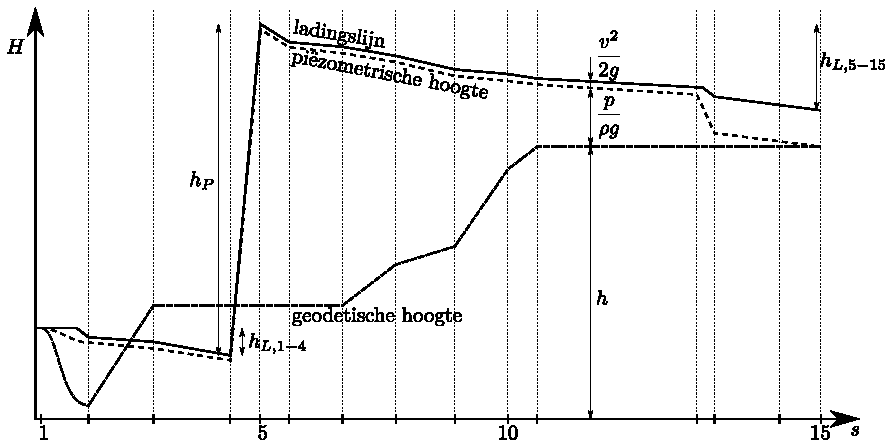
\includegraphics{fig/leidingstelsels/leidingstelsel_energiehoogte}
	\caption{Grafische weergave van de mechanische energievergelijking voor het leidingstelsel in Figuur \ref{fig:leiding_structuur}}
	\label{fig:leidingstelsel_energiehoogte}
\end{figure}


